\section*{}
\fbox{\parbox{\textwidth}{This tutorial explains the use of the "Point Spread Function Estimation Tool", implemented as a plugin for ImageJ. The plugin is still under active development. Your comments on functionality, design, and bugs are highly appreciated.}}

\section{General Description}
Your microscope setup constitutes an expensive and precious resource from which you want to get the best possible performance. Therefore, you should not rely on purely qualitative performance metrics like "it looks pretty good". Your eyes are not capable of telling the difference between a well-adjusted microscope and a poorly adjusted one.

In all real equipment, the imaging results are worse than the theoretically possible value (e.g.~by a factor of 1.5 in resolution). The reasons for this include imaging noise (prefer images with long exposure!), imperfections of the lenses, distortions caused by variations in cover slide thickness (your objectives are corrected for a specific thickness of slides and they are \emph{very} sensitive to this), the finite width of the emission wavelength spectrum (we also collect some light at longer wavelengths), point sources of finite extension, under-sampling due to a mismatch of magnification and camera pixel size, and so on. Or you might simply not have focused well enough. D'oh!

Most likely, many people in your lab share the use of a microscope. You can thus benchmark your results against the ones of your colleges to get a first clue about the quality of your images. The present tool gives you a quantitative way of doing so, enables you to adjust your microscope optimally, and to compare your images to the maximum possible theoretical quality. This is done on the basis of the microscope's \emph{Point Spread Function} (PSF).

The PSF is widely used to describe the imaging properties of optical systems such as light microscopes. Most importantly, the shape of the PSF is a measure for the resolving power of the optical system. In a nutshell, the PSF is the smeared image of a point-like source. The present tool is intended to be used for characterizing light microscopes (of any kind, e.g. fluorescence, wide-field, confocal, ...) equipped with a digital camera. With this tool you are able to estimate the PSF of a microscope setup and to compare it to the theoretical PSF as calculated from elementary parameters of the microscope and the camera. This serves two purposes: First, you might want to know whether you adjusted your equipment optimally, and second, the PSF can be used for image restoration purposes (in future versions of the plugin) such as deconvolution. 

Presently, this tool features:
%
\begin{itemize}
\item user-defined parameters,\\[-4ex]
\item free selection of images of point sources to be considered for PSF estimation,\\[-4ex]
\item automatic source position refinement based on intensity centroid estimation,\\[-4ex]
\item plots of the measured and the theoretical PSF, and\\[-4ex]
\item a report file containing all relevant input and output.
\end{itemize}

\section{Installation}
The plugin requires a working installation of ImageJ (version 1.36 or later) on your system. To install the plugin, simply drag the \texttt{mosaic\_plugins.jar} archive into the "plugins" folder of your local ImageJ installation. After restarting ImageJ, "PSF\_Tool" should be visible in the "Plugins$\rightarrow$ Mosaic" menu.

\section{How to use the Plugin}
In the following, we will walk through an example in order to describe the main features of the tool and their usage. We have, therefore, attached a sample image to the zip-file, called "sample.tif" (courtesy of Christoph Burckhardt, Greber lab, University of Zurich). The image shows endosomes and small vesicles in a human cell. While these objects are not strictly \emph{point sources}, they are still smaller than the resolution limit of the microscope (their size is about 100\,nm). For real applications, we strongly encourage you to spend some time on imaging small sources of known size, such as fluorescent beads, virus particles, quantum dots, or whatever is available in your lab. The smaller and brighter the better. Also consider that the sources should not move during exposure.

\subsection{Start and Configuration}
To start, open "sample.tif" in ImageJ. Currently, the plugin only handles 8-bit gray-scale images so we need to convert the Image. Select Image $\rightarrow$ Type $\rightarrow$ 8-bit in the menu.
Now start the plugin. A configuration dialog will appear (see Figure \ref{config}). Here, you have to enter necessary microscope, camera, and image parameters on which the calculations will be based.
\begin{figure}
\centering
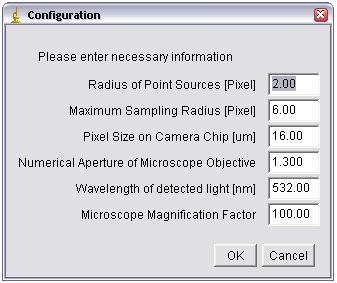
\includegraphics[scale=0.7]{config.jpg}
\caption{Configuration menu}
\label{config}
\end{figure}

\begin{description}
\item[Radius of Point Sources (pixel)] The apparent radius of the point sources in the image. The parameter is needed for position refinement. In our example, set it to 2.
\item[Maximum Sampling Radius (pixel)] Determines the radius around the centroid up to which the PSF is sampled. It is important to not set it below the first minimum of the PSF. Be conservative and set it to 4 in our example (which is twice the value of the apparent radius used above).
\item[Pixel Size on Camera Chip ($\mu$m)] Have a look at the data sheet of your microscope or camera. For the tutorial data this parameter is 16.
\item[Numerical Aperture of Microscope Objective] For the sample image the NA is 1.3.
\item[Wavelength of detected light (nm)] We imaged green fluorescent proteins and set the value to the emission maximum at 532\,nm.
\item[Microscope Magnification Factor] Overall microscope magnification factor. In our case 100.
\end{description}
Click "OK" after you have entered all parameters.

\subsection{Source Selection and PSF Estimation}
Once you have entered the configuration parameters, a GUI with 4 Buttons is displayed (see Figure \ref{gui}).
\begin{description}
\item[Start New Selection] Starts a new selection of point sources. Once pressed, every click on the image will result in a PSF estimation (be careful!).
\item[Enhance Contrast] Enhances Image Contrast by linearly re-scaling all pixel intensity values to the possible range from 0 to 255 using the following equation:
%
	\[
	I_{enhanced} = 255 * \frac{\left(I - \min\left(I\right)\right)}{\left(\max\left(I\right) - \min\left(I\right)\right)}
\]
%
 This does not affect the PSF estimation and is only done to enhance image viewing.
\item[Estimate PSF] Estimates the Point Spread Function from all selected sources.
\item[Create Report] Creates a text file containing all relevant result data.
\end{description}
\begin{figure}
\centering
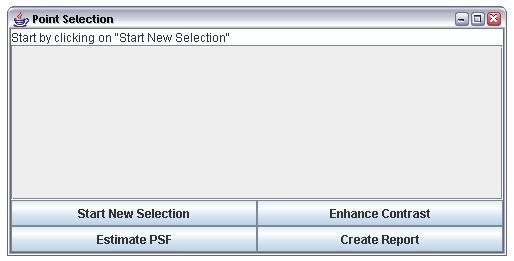
\includegraphics[scale=0.6]{gui.jpg}
\caption{Graphical User Interface (GUI)}
\label{gui}
\end{figure}
Let us now select some single-point sources. To make the selection more convenient, first zoom in to a specific area of the image using the ImageJ Magnifying Glass cursor. 

\begin{figure}[h]
  \center{
    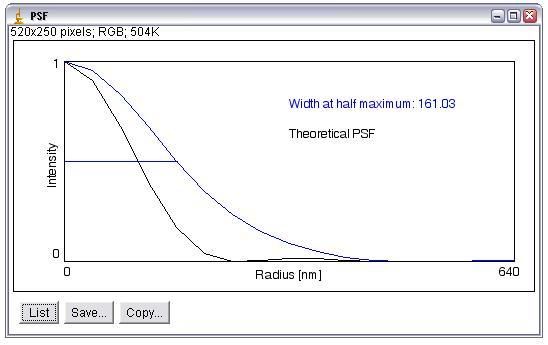
\includegraphics[scale=0.6]{psfplot.jpg}
  }
  \caption{Plot of Point Spread Function. The average intensity on concentric circles around the intensity centroid is plotted against the radius.}
  \label{plot}
\end{figure}

\begin{itemize}
\item Now click on "Start New Selection" and select some point sources in the image (make sure your cursor is set to single selection again after magnification!). Try to choose apparently small points (the less bright ones might be the smallest) outside noisy areas and without strong background variations and close neighboring sources. Also, make sure not to select spots that contain saturated pixels. This would render your PSF estimate meaningless! Each time you select a source, the position of the source is refined to sub-pixel accuracy (as described in \textit{I. F. Sbalzarini and P. Koumoutsakos. Feature Point Tracking and Trajectory Analysis for Video Imaging in Cell Biology, Journal of Structural Biology 151(2):182-195, 2005}) and a plot will show the estimated PSF of the last selection (see Figure \ref{plot}). Your selection is also added to the program's GUI and highlighted in the image by a red dot (see Figure \ref{selection}).

\begin{figure}[h]
\center{
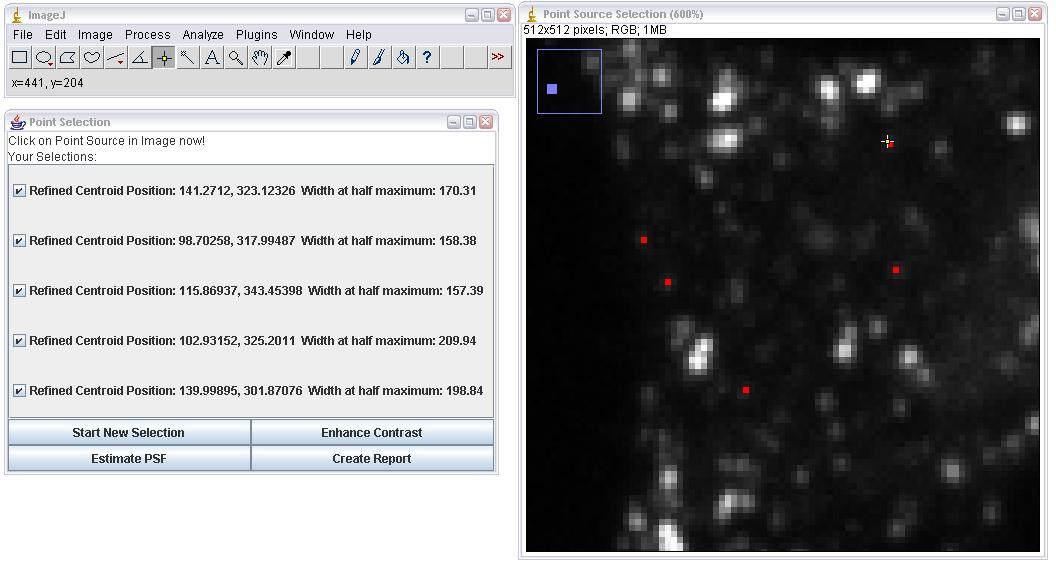
\includegraphics[scale=0.5]{selection.jpg}}
\caption{Point Source Selection}
\label{selection}
\end{figure} 
 
\item For each selection has its own checkbox in the GUI, stating the refined centroid position of the source and the width of the PSF at half maximum. Using these checkboxes you can select the sources that are to be considered for the overall PSF estimation.
\item To calculate the average PSF click "Estimate PSF". A new plot appears showing the average PSF. In addition, a theoretical PSF is calculated from the microscope and camera parameters. This allows you to compare the measurement with the theoretical curve. A good measure of comparison is the width at half maximum. The closer the measured PSF is to the theoretical one, the better the performance of your equipment. 
The theoretical PSF corresponds to the maximum possible resolution permitted by the laws of optics. It is computed from the wavelength $\lambda$ of the detected light, the microscope's numerical aperture $\mathrm{N\!A}$, and $C$ defining the intensity value at $r = 0$. Using the Bessel function $J_1(z)$, the theoretical PSF is then given by (as described in \textit{Y. Iketaki et. al. Theoretical investigation of the point-spread function given by super-resolving fluorescence microscopy using two-color fluorescence dip spectroscopy, Optical Engineering 44(3), 2005}):
	\[
	\mathrm{PSF}\left(r\right) = C\left[\frac{2J_1\left(\frac{2\pi}{\lambda}\mathrm{N\!A}r\right)}{\frac{2\pi}{\lambda}\mathrm{N\!A}r}\right]^2
\]
%
\item Click on "Create Report" in order to save the PSF data and the configuration parameters to a text file for later use or reference.
\end{itemize}

\section{Development and contact}
The present PSF tool is still under active development. It is currently limited to 2D-PSFs. If you are dealing with image z-stacks, you could either process them slice-by-slice to get an idea of z-resolution (I would not recommend this, however) or wait for a 3D version of our tool. Alternatively, you could make a maximum intensity projection using ImageJ's  "ZProjection" function. Note, however, that you will now measure the effect of your optical system \emph{plus} the projection! 

Please send comments, wishes, and reports to jo.helmuth@inf.ethz.ch or benedikt.baumgartner@inf.ethz.ch.
